% Copyright (c) 2015 Benito Palacios Sánchez - All Rights Reserved.
% Esta obra está licenciada bajo la Licencia Creative Commons Atribución 4.0
% Internacional. Para ver una copia de esta licencia, visita
% http://creativecommons.org/licenses/by/4.0/.

\section{Servicios en línea}
\subsection{Multijugador}
\begin{frame}[fragile]{Captura de paquetes}
\begin{columns}

\begin{column}{0.35\textwidth}
Estrategia \textit{man-in-the-middle}
\begin{center}
    \includefigure{\textit{Man-in-the-middle}}{imgs/man_middle.eps}
\end{center}
\end{column}

\begin{column}{0.5\textwidth}
\uncover<2->{Modificación DeSmuME.}
\begin{itemize}
    \item<3-> Paquetes PCAP.
\end{itemize}
\begin{uncoverenv}<3->\begin{lstlisting}
void create_packet();
void save_packet(u8* packet,u32 len);
void save_adhocPacket(u8* packet,
  u32 len, void* addr, bool isSent);
\end{lstlisting}\end{uncoverenv}

\begin{itemize}
    \item<4-> Exportar paquetes.
\end{itemize}
\visible<5->{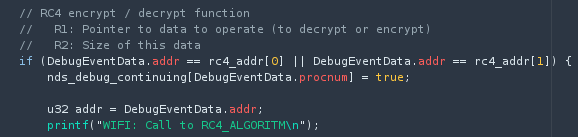
\includegraphics[width=\textwidth,keepaspectratio]{imgs/rc4exporter.png}}
\vfill
\visible<6->{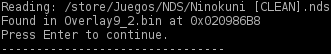
\includegraphics[width=\textwidth,keepaspectratio]{imgs/rc4finder.png}}
\end{column}

\end{columns}
\end{frame}

\begin{frame}{Servidores para Nintendo DS}

\begin{center}
    \visible<2->{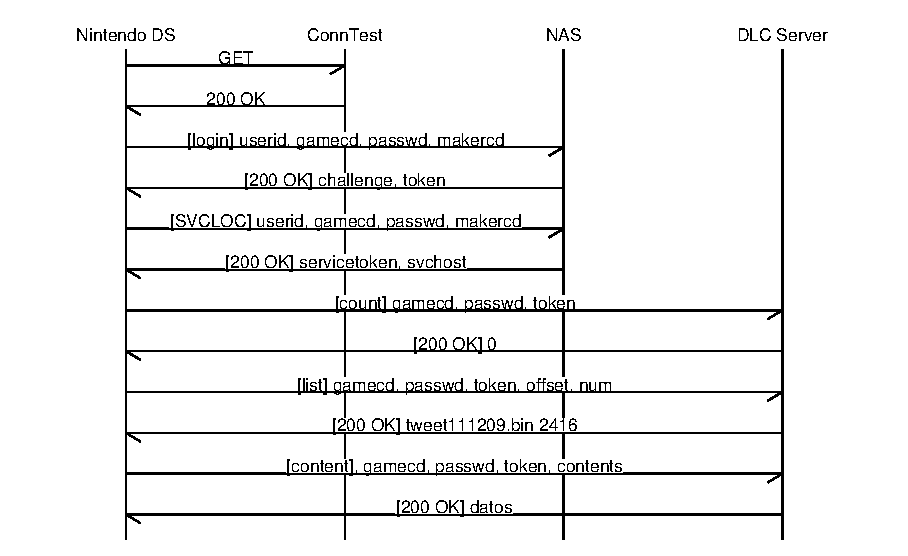
\includegraphics[width=\textwidth,height=0.5\textheight,keepaspectratio]{imgs/nds_dwc.eps}}
\end{center}

\uncover<3->{Vulnerabilidades:}
\begin{columns}
\footnotesize
\begin{column}{0.3333\textwidth}
    \begin{itemize}
        \item<4-> Puerto 80 del NAS abierto.
    \end{itemize}
\end{column}
\begin{column}{0.3333\textwidth}
    \begin{itemize}
        \item<5-> Contraseña no usada.
    \end{itemize}
\end{column}
\begin{column}{0.3333\textwidth}
    \begin{itemize}
        \item<6-> Autenticación simple.
    \end{itemize}
\end{column}

\end{columns}
\end{frame}

\begin{frame}{Preguntados}
\begin{columns}
    \begin{column}{0.15\textwidth}
        
\includegraphics[width=\textwidth,keepaspectratio]{imgs/preguntados_logo.png}
    \end{column}
    \begin{column}{0.85\textwidth}
        Trivial para plataformas móviles.
    \end{column}
\end{columns}

\begin{columns}
    \begin{column}{0.5\textwidth}
    \begin{itemize}
        \item<2-> Comunicación HTTP.
    \end{itemize}
    \end{column}

    \begin{column}{0.5\textwidth}
    \begin{itemize}
        \item<3-> Solución enviada antes de responder.
    \end{itemize}
    \end{column}
\end{columns}

\visible<4->{\includefigure{Preguntas, respuesta y solución de una partida}{imgs/preguntados_hack.png}}

\end{frame}

\subsection{Contenidos descargables}
\begin{frame}{Duet}
\begin{center}
\includegraphics[width=0.15\textwidth,keepaspectratio]{imgs/duet_logo.png}\end{center}

\begin{columns}
    \begin{column}{0.5\textwidth}
    \begin{itemize}
        \item<2-> Niveles extras por 0,99€.
        \item<4-> BD con preferencias sin proteger.
        \note<1>[item]{Es SQLite y se puede usar software como SQLiteMan}
    \end{itemize}
    \end{column}

    \begin{column}{0.5\textwidth}
    \begin{itemize}
        \item<3-> Ya incluídos pero desactivados.
        \item<5-> Se puede activar a mano.
    \end{itemize}
    \end{column}
\end{columns}

\visible<5->{\includefigure{Filas con estado de los contenidos extras}{imgs/duet-levels.png}}

\end{frame}

\begin{frame}{\textit{Download Play}}
Compartir demos con comunicación inalámbrica ad-hoc.

\uncover<2->{\underline{Problema:}}
\begin{columns}
    \begin{column}{0.5\textwidth}
    \begin{itemize}
        \item<3-> Envío de código de una consola a otra.
        \item<5-> El código principales se firman con \texttt{RSA}.
    \end{itemize}
    \end{column}

    \begin{column}{0.5\textwidth}
    \begin{itemize}
        \item<4-> Se podría interceptar y cambiar para acceder a la consola.
        \item<6-> Los módulos de código adicional no.
    \end{itemize}
    \end{column}
\end{columns}

\uncover<7->{\underline{Solución:}}
\begin{itemize}
    \item<8-> El archivo principal comprueba con \texttt{HMAC} los módulos.
    \item<9-> La clave y el resultado se guarda en este fichero.
    \item<10-> Solo si el inicio es \textit{Download Play} y no desde un cartucho.
\end{itemize}
\end{frame}
